% Project LEPTON: the paper (PJDSC 2026). Workstream E of lepton-plan.md.
%
% Build with pdfLaTeX and Biber (on Overleaf: Menu > Compiler > pdfLaTeX; Overleaf runs Biber
% by itself). paper/README.md says how, and which file holds which task.
% Each section is one file in sections/, its task code in the comment at its top.
% Text marked \checkme{...} still needs a teammate's check before submission (E11).
\documentclass[10pt, twocolumn]{article}
\usepackage{lepton}
\addbibresource{references.bib}

\hypersetup{
  pdftitle={Project LEPTON: Leptospirosis Exposure Prediction and Targeting Operational Network}}

\begin{document}

\twocolumn[{%
  {\leptonkicker PROJECT PAPER\par}
  \vspace{2mm}
  {\leptontitlefont Project LEPTON\par}
  \vspace{1mm}
  {\leptonsubtitlefont Leptospirosis Exposure Prediction \& Targeting Operational Network\par}
  % No team, school or author names: PJDSC's guidelines ask for none.
  \vspace{5mm}
  % E9 (SCRUM-60): Executive summary, written last (October 22): under 250 words, with D5's
% primary result in it. The keywords are the submitted proposal's.
\begin{leptonsummary}
{\color{leptonnavy}\large\bfseries EXECUTIVE SUMMARY\par}
\vspace{1mm}
\checkme{E9: written last, under 250 words, with the primary result (lepton-plan.md, E9).}

\vspace{1mm}
{\color{leptonnavy}\large\bfseries KEYWORDS\par}
\vspace{1mm}
Leptospirosis, infectious disease forecasting, time-series forecasting, flood exposure,
climate-sensitive disease, tropical cyclones, prophylaxis stock allocation, probabilistic
forecasting, public health preparedness, Philippines
\end{leptonsummary}
% E9 (and the keywords)
  \vspace{6mm}
}]

% E4 (SCRUM-25): Background. Starts from the submitted proposal's Background (lepton-plan.md,
% task E4). Every source was opened and checked on 2026-10-21.
% Numbers: QC's cases are QCESD's weekly counts by onset week (results/forecasts.csv, column y,
% weeks from epiweeks); 4,953 cases and the onset dates are in data/raw/qcesd.md; storm dates
% are config.STORMS (data/raw/storm-facts.md); the census total is config.CENSUS_POP_QC.
\section{Background}\label{sec:background}

Leptospirosis is a bacterial disease that people catch from animals. The bacteria spread
through the urine of infected animals, and people are infected through contact with water or
soil that holds it; the risk is higher after typhoons, heavy rain and floods
\parencite{cdc2026}. The Philippines has all three every year: an average of 20 tropical
cyclones enter the Philippine Area of Responsibility, and 8 or 9 of them cross the country
\parencite{pagasa_nd}. In Manila, weekly hospital admissions for leptospirosis from 2001 to
2012 rose with rainfall and peaked two weeks after it, and floods explained part of that rise
\parencite{matsushita2018}.

Quezon City (QC) is the most populous city in the country, with 3,084,270 residents in the
2024 census \parencite{psa_census2024}. Its low-lying barangays line the Marikina, San Juan
and Tullahan rivers, and floods on the Marikina are driven by rain over its upper watershed,
outside the city \parencite{abon2011}. The city's Epidemiology and Surveillance Division
(QCESD) recorded 4,953 leptospirosis cases with dates of onset from January 2015 to
mid-October 2026 \parencite{qcesd2026}. Its three largest surges each peaked one to two weeks
after a flood: 125 cases had their onset in the week of 4--10 August 2024, after Typhoon Carina
flooded the city on 23--25 July; 179 in the week of 27 July--2 August 2025, after the floods of
19--24 July; and 223 in the week of 23--29 August 2026, after the habagat (southwest monsoon)
floods of 8--11 August.

Time-series regression is a common design for relating weather to infectious-disease counts
over short lags \parencite{imai2015}. For leptospirosis in the Philippines,
\textcite{latigay2026} combined Prophet with XGBoost on national weekly counts
\parencite{parreno2023} and reported a lower forecast error than Prophet alone or a seasonal
naive forecast. They also observed that standard statistical models over-smooth surveillance
data: they capture the seasonal trend but miss the sharp peaks that define an outbreak.

The Department of Health (DOH) also recommends doxycycline prophylaxis for people exposed to
floodwater, sized to their exposure. Department Memorandum (DM) No.~\mbox{2023-0309} gives one dose after a
single exposure with no break in the skin, a 3- to 5-day course after exposure with a wound or
with floodwater in the eyes, nose or mouth, and a weekly dose while exposure is repeated or
continuous; children and pregnant women have regimens of their own, and a physician must be
consulted before any prophylaxis is given \parencite{doh2023}. Because each regimen follows
from a person's exposure, the stock a health center needs after a flood follows from how many
of its residents the flood reaches, and for how long.
   % E4
% E4 (SCRUM-25): The Problem. Starts from the submitted proposal's section; each of the two
% gaps below is one layer's reason for being (Layer 1: the forecast; Layer 2: the stock).
% Interior et al. (2025) is paraphrased: the proposal's sentence was almost their own words.
\section{The Problem}\label{sec:problem}

Two gaps keep these warnings from reaching the people who act on them.

The first is in forecasting. Standard statistical models follow the season but smooth over the
sudden spikes that severe weather triggers, and the published Philippine benchmark forecasts
from past counts and the calendar alone \parencite{latigay2026}, so it cannot see a flood
coming. A forecast that misses a surge gives hospitals and health offices no time to prepare.

The second is in the response. Philippine responses to leptospirosis remain mostly
hospital-based and reactive, and each rainy-season surge draws down hospital supplies and
budgets \parencite{interior2025}. Prophylaxis can be given only if the doses are at the health
center when exposed residents arrive, so the stock has to be in place before or just after
the flood. That needs an estimate, made from a rain forecast, of how many residents of each
barangay a storm will expose in each DOH risk group, and the published forecasting models do
not make one. Without it, prophylaxis cannot be placed ahead of the water, and the burden falls
hardest on the flood-exposed communities that need it most.

LEPTON addresses both gaps with one shared flood computation, rain set against flood hazard
maps and population counts. It feeds a city forecast that can see floods coming, one week
ahead, and barangay-level prophylaxis stock, one to three days before a storm. It is designed
for any Philippine city: every input except a city's case counts comes from a national or
global source. This study builds and tests it in Quezon City; Section~\ref{sec:scope-scope}
gives the reasons.
      % E4
% E3 (SCRUM-24): Objectives, from the submitted proposal (lepton-plan.md, E3).
\section{Objectives}\label{sec:objectives}

\checkme{E3: the objectives (lepton-plan.md, E3).}
   % E3
% E4 (SCRUM-25): Scope and Limitations.
% Scope = the core in lepton-plan.md's overview, as built: decision-tree row "QC weekly counts
% by onset week", option C, g = 2 (Notes.md 1.5); Kristine added as a fourth storm (Notes.md
% 1.1; confirmed for E4 on 2026-10-21). Limitations = every item the plan cut, plan corrections
% 1, 2, 8 and 9, the assumptions table (tables/assumptions.tex), Notes.md sections 1-3 and the
% decision tree's "say in the paper" line for option C.
% Numbers: results/forecasts.csv (454 forecasts per model, 349 in the MAE window, M3's 1,065
% for 2018 week 31, the 1.5-case threshold), results/c8_observed_runs.csv (Carina 120.0 mm,
% R0 119.7 mm, 1,414 exposed), results/m3_reproduction.md, data/raw/qcesd.md (207 published,
% 264 in the list, 17 days), data/raw/noah.md (11 barangays, 542 people), Notes.md 1.5
% (83, 163, 176 and 775 cases), results/m4_residual_acf.csv (M4's misses 1 and 2 weeks apart:
% 0.41 and 0.15, 95% band 0.08 and 0.09; python -m src.m4), config.py.
% Scope's first two paragraphs (October 23, at the team's request): LEPTON is designed for any
% Philippine city; QC came first as the most populous city (background.tex, psa_census2024) with
% an up-to-date case list (data/raw/qcesd.md: onset 2015-01-30 to 2026-10-14, received 20 October
% 2026), and because the schedule left time to request counts from one city only. The national
% fallback is the decision tree's last row (lepton-plan.md). NOAH's maps cover most provinces:
% 66 to 79, by return period (data/raw/noah_national.md). Every other source is in Appendix E.
% Future work, M2 and the two-week forecast (October 23): Implementation Plan v2 (9 October
% 2026), p. 16, defines M2 as "Prophet, yearly seasonality only, no regressors"; its pp. 28-29
% ("Observed versus forecast weather") score the two-week forecast on observed weather for the
% coming week, an optimistic upper bound (the plan's "ceiling run"), and on archived forecasts,
% and note that the one-week forecast uses observed weather only. The flag rule (25%, 50%) was
% confirmed by the team on October 23.
\section{Scope and Limitations}\label{sec:scope}

\subsection{Scope}\label{sec:scope-scope}

LEPTON is designed for any Philippine city, since every input but the case counts comes from a
national or global source (Appendix~\ref{app:sources}): IMERG, ERA5 and ECMWF rain, the WorldPop
grid, the PSA census and birth tables, the national barangay boundaries, the DOH facility
registry, the HydroBASINS river basins and Project NOAH's flood maps, which cover most provinces.
Another city therefore needs its own weekly case counts for Layer~1, and its catchments,
barangays and health centers, drawn from the same sources, for both layers; Layer~2 needs no
case data.

This study covers one city, Quezon City, for two reasons. First, QC is the country's most
populous city, and QCESD keeps an up-to-date list of the city's leptospirosis cases with each
case's date of onset, from January 2015 to mid-October 2026, which supports weekly forecasting.
Second, the competition's schedule left time to request case counts from one city only,
and a reply in time was not assured: without one, Layer~1 would have fallen back to national
weekly counts \parencite{parreno2023}, without flood features. QCESD's list arrived on 20 October
2026. Because only one city was tested, results may not carry over to cities with different
drainage, climate or reporting. Cases are counted by week of onset (CDC/MMWR weeks), and no
case-level record is published.

\emph{Layer 1} forecasts next week's number of cases in QC by week of onset, with a 90\% range
and the probability that the count exceeds the epidemic threshold, set here at the same week's
mean plus two standard deviations over up to five recent non-COVID years. Four models are
compared: two seasonal baselines, M0 (the count 52 weeks earlier) and M1 (the same week's
average over the threshold's years); the published Prophet--XGBoost hybrid, M3
\parencite{latigay2026}, first reproduced on its own national data \parencite{parreno2023}; and
the proposed negative binomial regression, M4, also refitted without its flood exposure index to
test whether flood exposure adds accuracy. In a weekly
rolling-origin backtest every model made 454 one-week-ahead forecasts, for the weeks from
14--20 January 2018 to 20--26 September 2026. The primary endpoint is M4's mean absolute error
against M3's over the 349 forecasts outside the COVID-19 years 2020--2021, with a 95\%
moving-block bootstrap interval \parencite{kunsch1989}.

\emph{Layer 2} counts, for each of QC's 142 barangays, the residents in each hazard level of
Project NOAH's 5-, 25- and 100-year flood maps \parencite{noah_nd}, from the WorldPop 2024
population grid \parencite{bondarenko2025} fitted to the 2024 census
\parencite{psa_census2024}. A storm's rain over the river catchments that drain into the city,
set against that rain's return levels, decides how many of those residents it exposes. The
exposed residents then become stock under DM~\mbox{2023-0309} \parencite{doh2023}: doxycycline 100~mg
capsules for adults by risk tier, courses for children and amoxicillin 500~mg tablets for
pregnant women, per barangay and per health center. These are stock-planning figures, not
prescriptions.

Layer 2 was run on four storms: Typhoon Carina (July 2024), Severe Tropical Storm Kristine
(October 2024), the July 2025 floods and the August 2026 habagat floods. Each ran on observed
satellite rain from NASA's IMERG \parencite{huffman2024} and on ECMWF forecasts issued one, two
and three days before its rain, from Open-Meteo's archive \parencite{zippenfenig2023}. Observed
rain is set against IMERG's own return levels and forecast rain against ERA5's
\parencite{hersbach2020}, because the two products differ in scale. Kristine was not in the
project proposal; it was added because IMERG puts Carina's rain at the no-flood floor
(Section~\ref{sec:limitations}), so Carina alone could not show the chain at work. Each run is
compared with the barangays that city and news reports named as flooded. LEPTON is meant as a
decision-support tool for health offices, not a replacement for clinical judgment.

\subsection{Limitations}\label{sec:limitations}

The limitations are grouped by the part of the study they affect. Table~\ref{tab:assumptions},
in Appendix~\ref{app:assumptions}, lists every assumption behind them, with its value and how it
was tested.

\paragraph{Case data}
QCESD's list gives each case's dates of onset and admission but not the date the case was
reported, so what the office knew on each forecast day cannot be rebuilt. Cases are therefore
forecast by week of onset from final counts and, at each forecast, the last two weeks of counts
are hidden from every model, as if they had not been reported yet. Two weeks is an assumption,
since QCESD's reporting delay is not known. The backtest therefore uses final counts with a
two-week guard, and real-time accuracy may be lower. Counts published during a surge show the
gap: QCESD's total for 1 January to 3 August 2025 was 207 cases \parencite{herriman2025}, while
the final list holds 264 cases admitted by then. A week counts as final once 17 days have
passed since it ended, because 99\% of cases were admitted within 17 days of onset; the delay
from admission to report is unknown, so this is a lower bound, and the weeks after 20--26
September 2026 are left out as still filling in. Without report dates, those weeks also cannot
be nowcast, a step a live system would need.

Surveillance data likely undercount leptospirosis. QC's early years are also small: 83, 163 and
176 cases in 2015--2017, against 775 in 2018. If fewer facilities reported then, the thresholds
and M1 forecasts that average over those years are too low; the first threshold of 2018 is 1.5
cases a week. The list's own morbidity-week column changes meaning between years, so every
week is taken from the date of onset. The COVID-19 years 2020--2021 carry an indicator in M4, are
not threshold reference years and are left out of headline scores; all years are also scored,
as a check (Section~\ref{sec:results-checks}). Leaving them out joins 2019 directly to 2022 in the block bootstrap, once in 349
weeks. Finally, large surges are few, and the three largest came in the last three years, so no
model has many outbreaks to learn from.

\paragraph{Rain and flood exposure}
Satellite rain under-reads typhoons. In five typhoon rain events in the Philippines, IMERG
considerably underestimated the rain that gauges recorded \parencite{aryastana2022}, and
calibrating it against Philippine gauges brings it closer to them \parencite{veloria2021}.
Carina shows the cost: on
IMERG, its wettest three days over the catchments total 120.0~mm, at the no-flood floor $R_0$
of 119.7~mm, so its observed-rain run exposes about 1,400 residents and sizes almost no stock,
even though QC's cases surged one to two weeks later. Gauge-calibrated products track
Philippine typhoon rain more closely \parencite{bagtasa2022}, but switching would mean a new
26-year download, and IMERG's Final run arrives about three and a half months late, too late
for August 2026. ERA5, whose return levels judge the forecasts, also underestimates the highest
observed totals, with its largest errors in the tropics \parencite{lavers2022}; because each product is
judged on its own scale, this moves where a forecast falls but favors neither run.

A storm is measured by its wettest three consecutive days of IMERG rain over the catchments,
from the daily product on UTC days rather than a rolling 24-hour maximum, which would need
about 440,000 half-hourly files. A single wettest day missed the long habagat floods of 2025
and 2026, so three-day totals are used and the single day is kept as a comparison. NOAH's maps do
not state the duration of the rain they were drawn for, so neither choice can be tied to the
maps. Return levels rest on 18 to 26 years of IMERG, depending on the year: in a simulation with
25 years of annual maxima, 90\% of fitted 25-year levels fell between 16\% below and 14\% above
the true value, which moves where a storm falls between the maps, and fewer years widen that
range. Below the floor $R_0 = 0.5\,\hat{R}(5)$, half the five-year rain, nobody counts as
exposed; it is a starting value, left untuned because tuning needs floods that the city's
disaster office has listed.

The flood maps are static scenarios, not observed floods. NOAH's 100-year map is a later release
whose flood shapes are thinner in places: in 11 barangays a rarer map puts fewer residents in
flood zones than the five-year map does, by at most 542 people (San Jose, on the 100-year map).
The maps are used as published. WorldPop's counts are modeled, from a release (R2025A) that
WorldPop calls an alpha, and the 2020 census's age shares are applied to 2024 totals. The flood
exposure index is therefore a proxy for exposure, not a measure of it.

\paragraph{Models and evaluation}
The benchmark's published gain could not be reproduced. Rebuilt on the benchmark's own national
data, the seasonal naive forecast matched all eight of the paper's published scores for it, so
the data and the scored weeks agree, and Prophet came within 4.4\% of its published mean
absolute error (24.73 against 23.68). The rebuilt hybrid's error, however, was 24.60 against
the published 16.72, about the same as Prophet alone, and none of the 75 XGBoost settings tried
came within 10\%. Training XGBoost also on the forecast weeks' own errors, which a real forecast
cannot know, gives errors like the paper's; whether that happened cannot be told without the
authors' code. M4 is therefore compared with the reproduction of M3, and 16.72 is not quoted as
M3's accuracy. Ported to QC, M3 is also fragile early in the backtest, when only 2015--2017 lie
behind it: it forecast 1,065 cases for the week of 29 July--4 August 2018, which had 58.

The epidemic threshold is a choice made for this study, and QCESD's method may differ. Only
one-week-ahead forecasts are made. M4's misses come in runs: in its fit on the last forecast day,
one week's miss is correlated with the next week's (0.41) and with the one after (0.15), both
outside the 95\% range expected if weeks were independent ($\pm0.08$ and $\pm0.09$), consistent
with the newest count M4 can read being three to four weeks older than the week it forecasts; the
moving-block bootstrap allows for such runs. Interval and breach scores start in 2022, because each model's forecast spread is
estimated from its own past forecasts, which need a warm-up.

\paragraph{Prophylaxis stock}
Stock is sized by the regimens of DM~\mbox{2023-0309} \parencite{doh2023}. Its moderate-risk
group, adults with a wound or with floodwater in the eyes, nose or mouth, cannot be counted from
any available data, so for short floods the share $w$ of exposed adults in it is reported at 0,
0.5 and 1; the first and last are bounds. A flood lasting two days or more makes every exposed
adult high risk, this study's reading of continuous exposure, tested at one and three days. The memo makes doxycycline, 4~mg
per kg up to 200~mg, the first-line regimen for every child, so children are counted in courses
that a pharmacy turns into tablets by weight. Pregnant women's stock is amoxicillin 500~mg twice
a day for three days, from section II.B.2.b of the memo; PhilHealth's 2012 recommendations give
no prophylaxis regimen for pregnant women \parencite{philhealth2012}, so this regimen rests on
the memo alone, and women allergic to penicillin, who take erythromycin instead, are not stocked
separately. Lactating women are not counted apart from other adults: the census tables cannot
count them, and the memo gives them no regimen.

Pregnant women are estimated as 0.75 times the registered births to mothers living in QC, split
among barangays by their share of women aged 15--49; the registrations are not adjusted for
under-registration \parencite{psa_births2026}. Every resident of a flooded zone is counted as
touching the water, at any depth, and stock is reported at full coverage; a health office scales
the totals by the share of residents it expects to reach. Flood durations come from city and news
reports and may be off by a day (tested at $\pm1$ day); Kristine's one-day flood rests on
reports from 24 October only. A forecast cannot know how long the flood will last, so the
forecast runs report a one-day and a seven-day flood. Nor can it know when the rain will peak:
each lead takes the forecast's wettest three-day window among those ending on the storm's
observed wettest days, a choice made with hindsight. A live system would scan every window the
forecast covers and could pick other days and another amount, so the forecast runs show what
the forecasts said about the storm's own days, not the trigger an office would have seen.
Stock goes to the 66 health centers that
the national facility registry places inside their own barangays; the City Health Office is
treated as holding the city's stock rather than handing it out.

Finally, Layer 2 is checked against flood reports, not against cases. The reports name 8 to 17
flooded barangays per storm and are incomplete, and a barangay counts as flagged when at least
25\% of its residents live in zones the rain floods (50\% is also reported), a line chosen
because every barangay has some residents in the five-year zones. The storm runs are therefore
demonstrations, not
validations: no barangay case counts were used, and four storms are too few to measure forecast
error. LEPTON estimates stock needs, not supply chains, delivery or uptake, and every dose
figure in this paper is a stock-planning figure, not a prescription: DM~\mbox{2023-0309} requires a
physician's consultation before any prophylaxis.

\subsection{Not Covered: Future Work}\label{sec:future}

To finish within the competition's schedule, several parts of the project's original plan were
cut. They are named here so that no result is read as covering them:
\begin{itemize}
  \item other Philippine cities, Cebu City first, each with its own weekly case counts
    (Section~\ref{sec:scope-scope});
  \item running LEPTON live each week, which needs counts as they arrive and report dates to
    nowcast the weeks still filling in;
  \item forecasting cases two weeks ahead. The one-week forecast reads only rain that has
    already fallen; a two-week forecast could also use the coming week's rain from a rain
    forecast, and would then be scored twice, on the rain that fell (an optimistic upper bound)
    and on the archived forecasts that existed on each forecast day;
  \item two more models for comparison: Prophet with yearly seasonality only (M2) and an
    XGBoost model (M5);
  \item other population and flood maps: Meta's population map and the LiDAR-based flood maps
    on LiPAD;
  \item the full sensitivity analysis, of which only the tests in Table~\ref{tab:assumptions}
    were run;
  \item tuning the no-flood floor $R_0$ on floods the city's disaster office has listed;
  \item a distributed-lag non-linear model of rain and cases;
  \item checking flagged barangays against satellite flood maps (Sentinel-1) and against
    barangay case counts; and
  \item forecasting hospital demand.
\end{itemize}
        % E4
% E5 (SCRUM-56): Methodology, as built: QC only; M0, M1, M3, M4; the decision-tree row used
% (option C, g = 2); observed and forecast rain on the storms. No formula in the main text;
% formulas go in the appendix (lepton-plan.md, E5).
\section{Methodology}\label{sec:methodology}

\checkme{E5: the methodology (lepton-plan.md, E5).}
  % E5
% E6 (SCRUM-57): Results: D5's primary result in one sentence with its interval, the score
% table, the flood test, the storm runs (observed and forecast) and D8's figures
% (lepton-plan.md, E6). Every number from results/.
\section{Results}\label{sec:results}

\checkme{E6: the results (lepton-plan.md, E6).}
      % E6

\printbibliography            % E7: references.bib, APA 7th edition

% E8 (SCRUM-59): Appendices: Figures 1 and 1b updated to the core scope, the model table, the
% assumptions table (from E4), E5's formulas and the data sources with download dates
% (lepton-plan.md, E8).
% E8 sets their order; \appendix numbers their tables A1, B1, ... (lepton.sty).
% Figures A1 and A2 are the Methodology document's (9 October 2026) Figure 1 and its next
% diagram, the Layer 1 pipeline, redrawn as built by src/diagrams.py (python -m src.diagrams,
% copied from results/e8_fig_*.png). The model table follows config.py, src/baselines.py,
% src/m3.py, src/m4.py and src/forecast_range.py; the data sources table, the notes in data/raw/.
\clearpage
\onecolumn
\appendix

\section{Study Design}\label{app:design}

\begin{figure}[h]
\centering
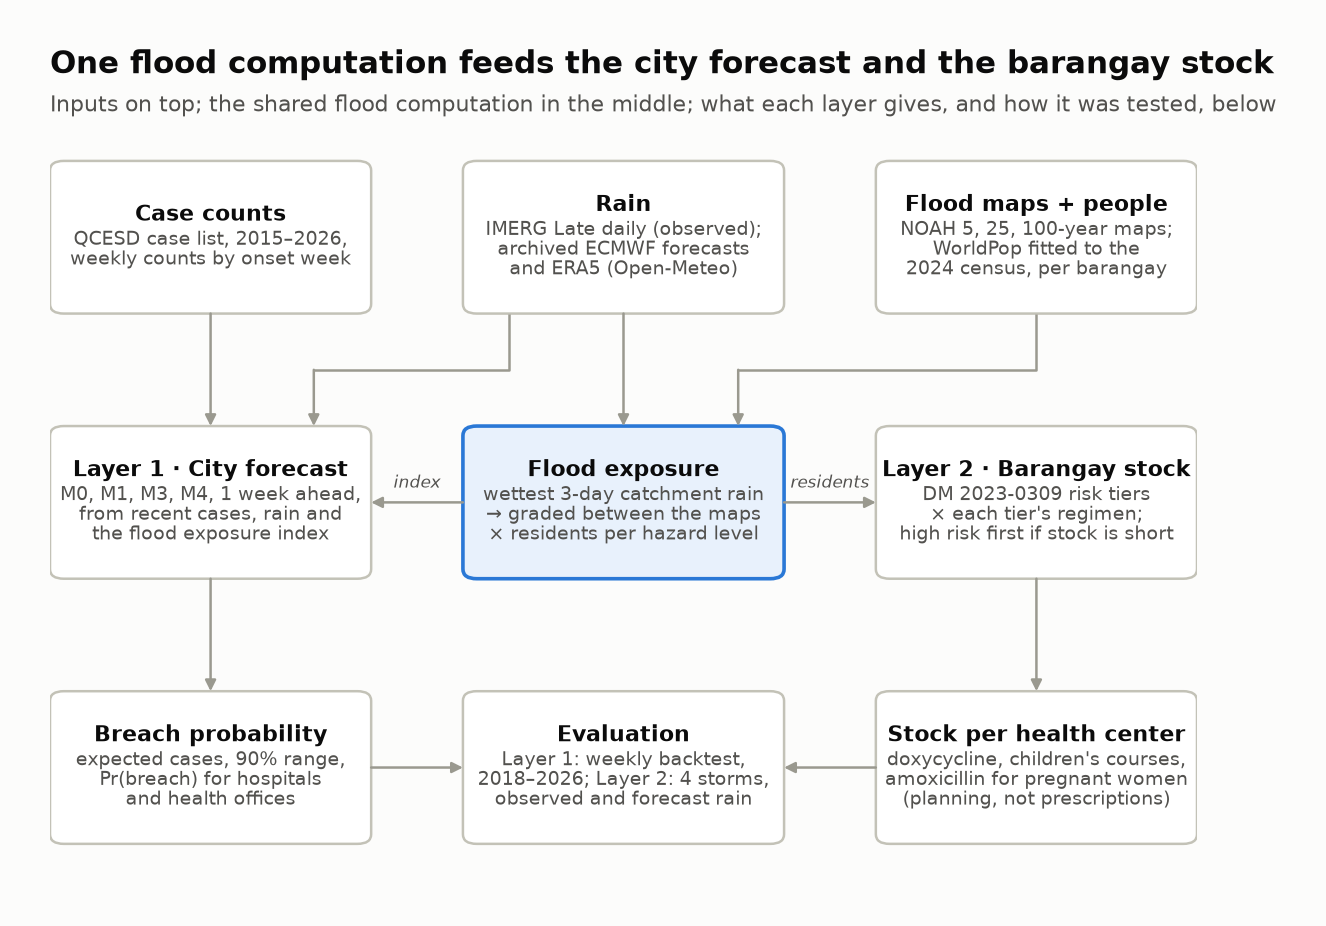
\includegraphics[width=0.94\textwidth]{figures/e8_fig_design.png}
\caption{The study design, updated from the project's methodology to what was built: QC only,
weekly counts by week of onset, four models forecasting one week ahead, rain measured over three
days, and Layer~2 checked on four storms. The flood computation (blue) turns rain into exposed
residents for Layer~2 and into the flood exposure index for Layer~1. Stock figures are for
planning, not prescriptions.}\label{fig:design}
\end{figure}

\begin{figure}[h]
\centering
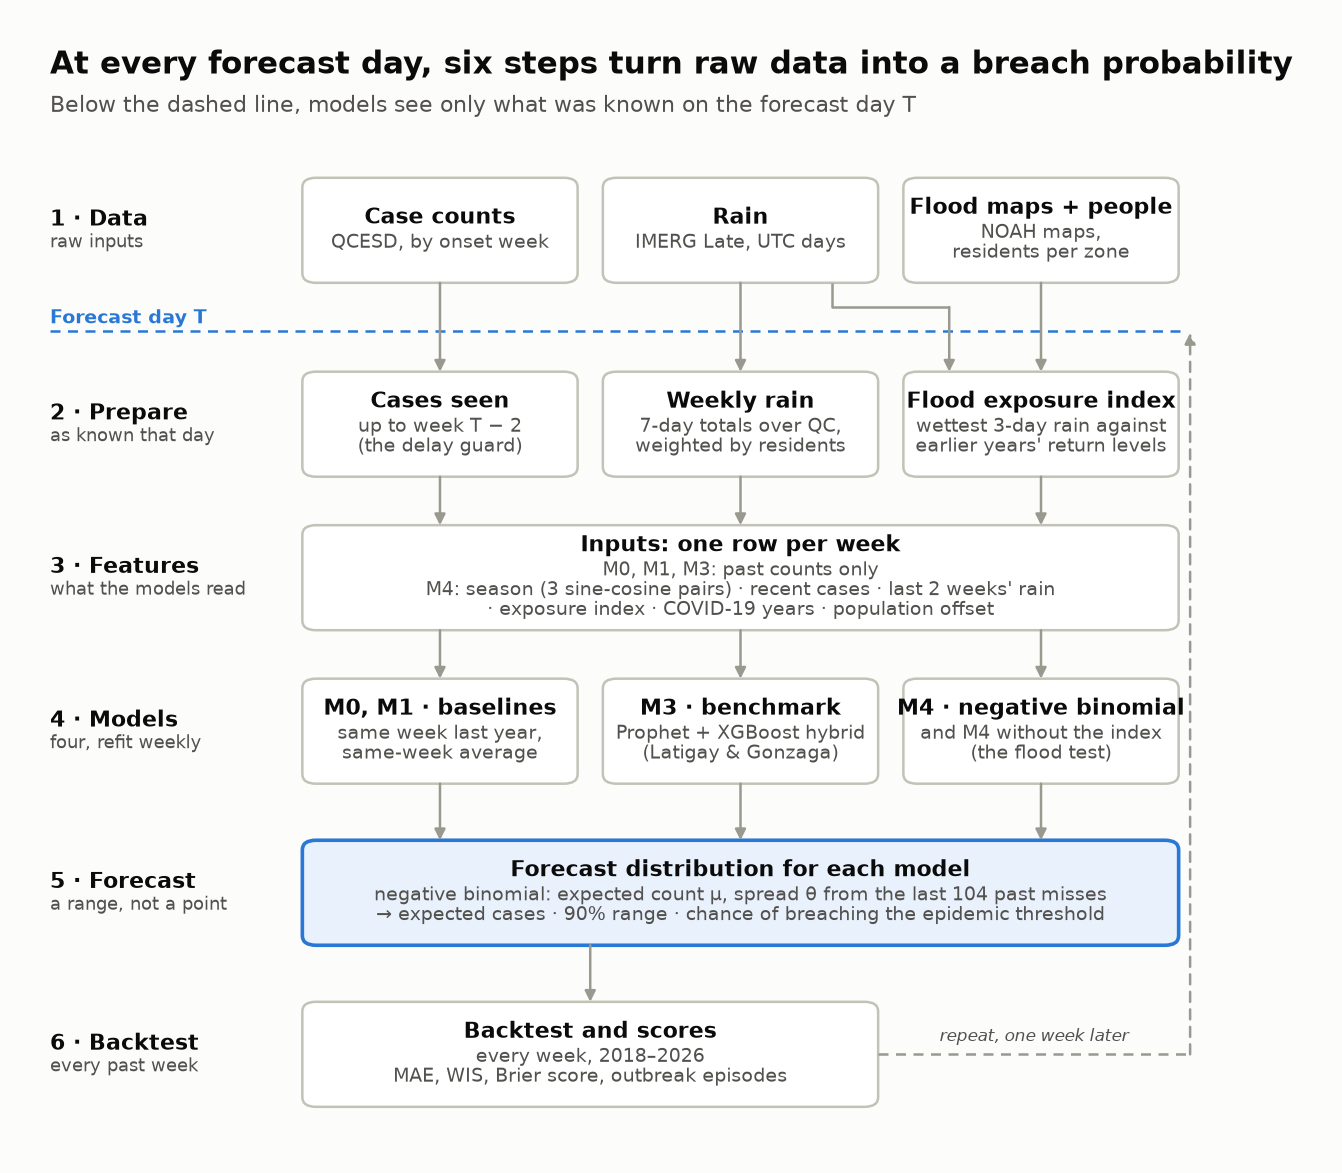
\includegraphics[width=0.94\textwidth]{figures/e8_fig_layer1.png}
\caption{Layer~1's steps at every forecast day. Rain and the flood exposure index are known on the
forecast day; case counts only up to two weeks before it (the delay guard). The backtest repeats
the six steps once a week, refitting every model each time.}\label{fig:layer1}
\end{figure}

\clearpage
\section{Models}\label{app:models}

{\footnotesize
\renewcommand{\arraystretch}{1.25}
\begin{longtable}{@{}>{\raggedright\arraybackslash}p{0.13\textwidth}
                    >{\raggedright\arraybackslash}p{0.26\textwidth}
                    >{\raggedright\arraybackslash}p{0.29\textwidth}
                    >{\raggedright\arraybackslash}p{0.24\textwidth}@{}}
\caption{The four models of Layer~1 and the flood test's variant. Each forecasts the count of the
week after the forecast day from what the delay guard lets it see, and is refitted at every
forecast day. The formulas are in Table~\ref{tab:formulas}; the file that computes each model is
named in small type.}\label{tab:models}\\
\toprule
\textbf{Model} & \textbf{Forecast} & \textbf{Inputs and fit} & \textbf{Role} \\
\midrule
\endfirsthead
\multicolumn{4}{@{}l}{\textit{Table~\thetable, continued}}\\
\toprule
\textbf{Model} & \textbf{Forecast} & \textbf{Inputs and fit} & \textbf{Role} \\
\midrule
\endhead
\midrule
\multicolumn{4}{@{}r}{\textit{Continued on the next page}}\\
\endfoot
\bottomrule
\endlastfoot
M0, last year \cfg{baselines.py}
  & The count of the same week 52 weeks earlier
  & Past counts only; nothing is fitted
  & Baseline: what a health office knows without a model \\
M1, seasonal average \cfg{baselines.py}
  & The mean count of the same week of the year over the epidemic threshold's reference years
    (up to the five most recent complete years before the target year, at least three, without
    2020--2021)
  & Past counts only; nothing is fitted
  & Baseline, and the practical test: M4 must beat the usual week \\
M3, Prophet--XGBoost \cfg{m3.py, m3_port.py}
  & Prophet's forecast plus XGBoost's correction of it, floored at zero
  & Past counts. Prophet: multiplicative seasonality, changepoint prior scale 0.55, weekly and
    yearly seasonality, no holidays. XGBoost: Prophet's in-sample errors from Prophet's forecast
    and the ISO week; xgboost's defaults, 100 rounds
  & Benchmark \parencite{latigay2026}, rebuilt on its own national data before the port to QC;
    D5's primary endpoint compares M4 with it \\
M4, negative binomial \cfg{m4.py}
  & The expected count $\mu$ of a negative binomial regression with QC's population as an offset
  & Season (three yearly sine--cosine pairs), recent cases (the two newest counts it may see),
    the last two weeks' rain over QC, the flood exposure index (larger of the last two weeks'),
    the COVID-19 years. Maximum likelihood with statsmodels' \texttt{negativebinomial}, which
    estimates the overdispersion; a term constant in every training row is left out
  & The proposed model \\
M4 without the index \cfg{m4.py}
  & As M4
  & M4's inputs without the flood exposure index, on the same rows
  & The flood test: does the index help? \\
\midrule
Every model \cfg{forecast_range.py}
  & A negative binomial with mean $\mu$ and spread $\theta$: expected cases, 90\% range and
    Pr(breach)
  & $\theta$ from the model's last 104 forecasts outside 2020--2021 whose counts it may see;
    with fewer than 26, its training fit's (M4: $1/\alpha$; M3: Prophet's); Poisson when misses
    are no wider than Poisson's
  & Makes every model's ranges and breach probabilities comparable \\
\end{longtable}
}

\clearpage
\section{Assumptions}\label{app:assumptions}
% E4 (SCRUM-25): the assumptions table, which E4's limitations point to; E8 places it among the
% appendices. Rows = the 29 assumptions in lepton-plan.md ("Assumptions to state in the paper"),
% less option A's reported-share cut-off (not used: A13 chose option C), plus the choices the
% build added (Notes.md sections 1-2 and config.py). Each value is the one in config.py; the
% config.py name sits under each assumption. Task codes are in the comment at each row's end.
% A test marked \checkme has not been run yet: run it, or change the cell to "Stated".
{\footnotesize
\renewcommand{\arraystretch}{1.18}
\begin{longtable}{@{}>{\raggedright\arraybackslash}p{0.22\textwidth}
                    >{\raggedright\arraybackslash}p{0.43\textwidth}
                    >{\raggedright\arraybackslash}p{0.29\textwidth}@{}}
\caption{Every assumption in LEPTON, its value and how it was tested. Values are set once, in
the code's \texttt{config.py}, under the names shown in small type.}\label{tab:assumptions}\\
\toprule
\textbf{Assumption} & \textbf{Value} & \textbf{Tested or stated} \\
\midrule
\endfirsthead
\multicolumn{3}{@{}l}{\textit{Table~\thetable, continued}}\\
\toprule
\textbf{Assumption} & \textbf{Value} & \textbf{Tested or stated} \\
\midrule
\endhead
\midrule
\multicolumn{3}{@{}r}{\textit{Continued on the next page}}\\
\endfoot
\bottomrule
\endlastfoot
%
\multicolumn{3}{@{}l}{\textbf{\color{leptonnavy}Cases and the city forecast (Layer 1)}}\\
A case's week \cfg{QCESD_ONSET}
  & The MMWR week of its date of onset; the list's own morbidity-week column is not used
  & Stated: that column changes meaning between years \\ % A13
Delay guard \cfg{DELAY_GUARD_G}
  & 2 weeks: forecasting week $T+1$ at week $T$, every model sees counts up to week $T-2$
  & Rerun with 1 and 3 weeks: the same three verdicts (Table~\ref{tab:robustness}) \\ % B2, B6, D3, D4
When a week's count is final \cfg{CASES_COMPLETE_DAYS}
  & 17 days after the week ends; later weeks are missing, not zero
  & 99\% of cases were admitted within 17 days of onset; a lower bound, since the delay from
    admission to report is unknown \\ % A13
Repeated rows in the case list
  & The 136 rows that repeat another row are kept as separate cases
  & With them the list matches QCESD's published 2025 totals to within 1\% \\ % A13, S4
Epidemic threshold \cfg{THRESHOLD_SD}
  & The week's mean plus 2 standard deviations over the up to 5 most recent complete non-COVID
    years before the target year, at least 3
  & Stated; QCESD's own method is not known \\ % B7
Week 53 \cfg{MAX_WEEK}
  & Treated as week 52; a reference year's own week 53 is not used
  & Stated \\ % A3, B7, B8
COVID-19 years \cfg{COVID_YEARS}
  & 2020--2021: an indicator in M4; not threshold reference years; out of headline scores
  & Every score also computed over all years, as a check (Section~\ref{sec:results-checks})
    \\ % B5, B7, D
Forecast spread before 26 past forecasts \cfg{THETA_MIN_FORECASTS}
  & Each model's training fit: M4's fitted $\theta$; M0's and M1's own fits on the weeks they
    see; Prophet's in-sample fit for M3
  & Stated; used for about the first half of 2018 only \\ % B6, B9, B10
M3's XGBoost settings \cfg{M3_XGB_PARAMS}
  & xgboost's defaults with 100 rounds; the paper gives none
  & Rerun with a maximum depth of 2: hybrid error 26.04 on the paper's data \\ % B3, B9
M3's gap filling \cfg{M3_LOCKDOWNS}
  & Our reading of the paper's three steps: lockdown weeks are those under ECQ or MECQ
    (15 March--31 May and 4--18 August 2020), and the series has no row for ISO 2020 week 53
  & Our seasonal naive forecast then matches all eight of the paper's published scores for it
    \\ % B3
\midrule
\multicolumn{3}{@{}l}{\textbf{\color{leptonnavy}Rain and flood exposure}}\\
Trigger rain \cfg{RAIN_ACCUM_DAYS}
  & The wettest three consecutive UTC days of daily IMERG Late rain
  & The single wettest day, run as a comparison \\ % A4, C3
A storm's rain
  & Its wettest three-day total ending during the flood
  & Stated \\ % C8, C9 (Notes.md 2.2)
Rain area \cfg{CATCHMENT_OUTLETS}
  & HydroBASINS level-12 sub-basins draining to the Marikina, San Juan and Tullahan rivers, each
    rain cell weighted by its area inside them
  & Stated \\ % A7, C3
IMERG's first year \cfg{IMERG_KEEP_2000}
  & June--December 2000 kept
  & Refit without it: return levels move by under 1~mm, the exposure index by at most 0.1
    point \\ % C3
Return-level fit \cfg{GUMBEL_MIN_YEARS}
  & Gumbel, on the annual maxima of at least 10 years before the forecast or storm year,
    refitted each year
  & Stated \checkme{the plan's one GEV refit for Carina was not run} \\ % C3
No-flood floor $R_0$ \cfg{R0_FACTOR}
  & $R_0 = 0.5\,\hat{R}(5)$, fixed
  & Stated; tuning it is future work \\ % C3
ERA5 fit years \cfg{ERA5_YEARS}
  & June 2000 to the year before each storm, the same years as IMERG
  & Stated \\ % A14, C9
Forecast model and lead times \cfg{FORECAST_LEADS_DAYS}
  & ECMWF IFS 0.25\textdegree, issued 1, 2 and 3 days before the rain
  & All four storms are in the archive \\ % A15, C9
Overlay rule
  & A pixel's residents count in proportion to its area inside a zone
  & Stated \\ % C2
Population map
  & WorldPop 2024, constrained 100~m (R2025A), fitted to each barangay's 2024 census total
  & Stated; Meta's map is future work \\ % A6, C1
Flood maps \cfg{NOAH_RETURN_PERIODS}
  & NOAH's 5-, 25- and 100-year Metro Manila maps, as published
  & The 11 barangays where a rarer map floods fewer residents were listed and inspected \\ % A8, C2
\midrule
\multicolumn{3}{@{}l}{\textbf{\color{leptonnavy}People and prophylaxis stock (Layer 2)}}\\
Age structure \cfg{CHILD_AGES}
  & The 2020 census's age shares, applied to 2024 totals
  & Stated \\ % C4
Pregnant women \cfg{PREG_BIRTHS_FACTOR}
  & 2024 registered births to mothers living in QC $\times$ 0.75, split among barangays by
    their share of women aged 15--49
  & 0.79\% of QC's residents, below the 3.5\% upper bound \\ % C4
Contact and uptake \cfg{CONTACT_SHARE_Q}
  & Every resident of a flood zone touches the water ($q = 1$) and takes prophylaxis ($u = 1$)
  & Stated; a health office scales the totals \\ % C5
Contact by hazard level \cfg{CONTACT_BY_LEVEL}
  & The same at every level ($r_k = 1$)
  & Stated \\ % C5
Adults with a wound or mucosal exposure \cfg{WOUND_SHARE_W}
  & A share $w$ of 0, 0.5 and 1 of exposed adults, in floods shorter than the cut-off below
  & 0 and 1 are the bounds \\ % C5
Continuous exposure \cfg{CONTINUOUS_EXPOSURE_DAYS}
  & A flood of 2 days or more makes every exposed adult high risk
  & Rerun at 1 and 3 days \\ % C5, C8
Moderate-risk course \cfg{MODERATE_COURSE_DAYS}
  & 5 days, the upper end of the memo's 3 to 5
  & Stated as a planning upper bound \\ % C6
Flood duration $D$ \cfg{STORMS}
  & From city and news reports: Carina 3, Kristine 1, July 2025 6 and August 2026 4 days
  & Rerun at $D \pm 1$ day \\ % A11, C5, C8
Flood duration in forecast runs \cfg{FORECAST_RUN_D}
  & $D = 1$ and $D = 7$ days, both reported
  & The observed $D$ shown beside them \\ % C9
Lactating women
  & Not separated from other adults
  & Stated: the memo gives them no regimen \\ % C6
Distribution points \cfg{CENTER_FACILITY_TYPES}
  & Health centers and barangay health stations, not the City Health Office
  & Stated \\ % C7
Barangays with several health centers, or none
  & Several: split by the residents living nearest each center; none: the nearest center, at
    most 2.04~km away
  & Stated \\ % C7
Flagged barangay \cfg{FLAG_EXPOSED_SHARES}
  & At least 25\% of its 2024 residents live in zones the storm's rain floods
  & Also reported at 50\% \checkme{the team confirms the rule, Notes.md 1.2} \\ % C8, C9
\midrule
\multicolumn{3}{@{}l}{\textbf{\color{leptonnavy}Evaluation}}\\
Bootstrap blocks \cfg{BOOT_BLOCK_WEEKS}
  & 8-week blocks, 2,000 resamples
  & Rerun with 4- and 13-week blocks \\ % D5, D6
Base rate for the Brier skill score
  & The share of non-COVID weeks from 2018 to the guard's cutoff that breached
  & Stated \\ % D3
Alarm cut-off $p^{*}$
  & The best F1 score on the first half of the forecast days
  & The full precision--recall curve, reported in Section~\ref{sec:results-layer1} \\ % D3
Outbreak episode \cfg{EPISODE_GAP_WEEKS}
  & Breach weeks at most 2 weeks apart form one episode
  & Stated \\ % D3
Surveillance delay, for lead time \cfg{DELAY_GUARD_G}
  & A breach shows in surveillance 2 weeks after its week, as in the delay guard
  & Stated \\ % D4
\end{longtable}
}


\clearpage
\section{Formulas}\label{app:formulas}
% E5 (SCRUM-56): the formulas behind the methodology, which keeps none in its text
% (lepton-plan.md, E5). One row per step, in the methodology's order; under each step, the file
% in src/ that computes it. Symbols as in that code, except the interpolation anchors (lo, hi),
% renamed so that b is always a barangay. Values (0.75, 52.18, 50, 104, 26, 11 ranges, 8-week blocks) are config.py's.
{\footnotesize
\renewcommand{\arraystretch}{1.4}
\setlength{\lineskiplimit}{1pt}% stacked sub- and superscripts on two lines of a cell
\setlength{\lineskip}{3pt}%      never touch: TeX puts 3pt between them instead
\begin{longtable}{@{}>{\raggedright\arraybackslash}p{0.19\textwidth}
                    >{\raggedright\arraybackslash}p{0.43\textwidth}
                    >{\raggedright\arraybackslash}p{0.32\textwidth}@{}}
\caption{The formula behind each step of the methodology (Section~\ref{sec:methodology}), in
its order. The file in the repository's \texttt{src/} folder that computes it is named in small
type under each step.}\label{tab:formulas}\\
\toprule
\textbf{Step} & \textbf{Formula} & \textbf{In plain words} \\
\midrule
\endfirsthead
\multicolumn{3}{@{}l}{\textit{Table~\thetable, continued}}\\
\toprule
\textbf{Step} & \textbf{Formula} & \textbf{In plain words} \\
\midrule
\endhead
\midrule
\multicolumn{3}{@{}r}{\textit{Continued on the next page}}\\
\endfoot
\bottomrule
\endlastfoot
%
\multicolumn{3}{@{}l}{\textbf{\color{leptonnavy}Shared flood computation}}\\
Population map fitted to the census \cfg{rescale.py}
  & $p'_i = p_i \, P_b \big/ \sum_j f_j(b)\, p_j$
  & The census sets how many live in barangay $b$ ($P_b$, 2024); WorldPop sets where ($p_i$ in
    pixel $i$); $f_j(b)$ is the share of pixel $j$ inside $b$ \\
Residents per flood zone \cfg{overlay.py}
  & $\mathrm{Pop}_{b,k,T} = \sum_i f_i(b \cap H_{k,T})\, p'_i$
  & Residents of $b$ in hazard level $k$ of the $T$-year map; a pixel half inside the zone
    counts half its people \\
Catchment rain \cfg{flood_exposure.py}
  & $R^{24}_d = \sum_g a_g\, R_{g,d}$, \quad $R^{3}_d = R^{24}_{d-2} + R^{24}_{d-1} + R^{24}_d$
  & IMERG's rain on UTC day $d$, each cell $g$ weighted by its share $a_g$ of the catchment
    area; a storm is its wettest three-day total \\
Return levels \cfg{flood_exposure.py}
  & $\hat{R}(T) = \mu - \beta \ln\!\left[-\ln\left(1 - 1/T\right)\right]$, \quad
    $R_0 = 0.5\,\hat{R}(5)$
  & Gumbel curve fitted by maximum likelihood to each year's wettest three-day total, on years
    before the forecast or storm year only \\
A storm's return period \cfg{observed_run.py}
  & $T_{\mathrm{storm}} = 1 \big/ \left[1 - F(R)\right]$
  & $F$ is the fitted curve's cumulative probability: rain this heavy comes about once in
    $T_{\mathrm{storm}}$ years \\
Graded exposure \cfg{flood_exposure.py}
  & $N_{b,k} = \mathrm{Pop}^{\mathrm{lo}}_{b,k} + \dfrac{R - R^{\mathrm{lo}}}{R^{\mathrm{hi}} -
    R^{\mathrm{lo}}} \left(\mathrm{Pop}^{\mathrm{hi}}_{b,k} - \mathrm{Pop}^{\mathrm{lo}}_{b,k}\right)$
  & Between the two anchors that bracket the rain $R$: $(R_0, 0)$, $(\hat{R}(5),
    \mathrm{Pop}_5)$, $(\hat{R}(25), \mathrm{Pop}_{25})$, $(\hat{R}(100), \mathrm{Pop}_{100})$;
    nobody below $R_0$, the 100-year map above $\hat{R}(100)$ \\
Flood exposure index \cfg{flood_exposure.py}
  & $\mathrm{EI}(t) = 100 \times \sum_b \sum_k N_{b,k}\!\left(R^{\max}_t\right) \big/
    P^{2024}_{\mathrm{QC}}$
  & Percent of QC's residents in zones that week $t$'s wettest three-day total $R^{\max}_t$
    would flood; over QC's 2024 total, never that week's population \\
\midrule
\multicolumn{3}{@{}l}{\textbf{\color{leptonnavy}Layer 1: city forecast}}\\
Population each week \cfg{population.py}
  & $P(t) = P_0 \left(P_1 / P_0\right)^{(t - t_0)/(t_1 - t_0)}$
  & Constant-percentage growth between the 2015, 2020 and 2024 censuses ($t$ in decimal years);
    the 2020--2024 rate after mid-2024 \\
Rain over QC \cfg{features.py}
  & $R_d = \sum_g v_g\, R_{g,d} \big/ \sum_g v_g$, \quad $R(t) = \sum_{d \in t} R_d$ \newline
    $\mathrm{Rcum2}(t) = R(t-1) + R(t)$, \quad
    $\mathrm{EI2}(t) = \max\left[\mathrm{EI}(t-1), \mathrm{EI}(t)\right]$
  & Each IMERG cell weighted by the residents $v_g$ it holds inside QC; a week's rain is the sum
    of its seven UTC days \\
What a model may see \cfg{view.py}
  & cutoff $= T - g$, \quad $\tilde{y}_{T+1} = y_{T-g} + y_{T-g-1}$ \newline
    training row for target week $s$: \ $\tilde{y}_s = y_{s-1-g} + y_{s-2-g}$
  & At forecast day $T$ the delay guard $g = 2$ hides the two newest weeks' counts; every
    training row keeps the same gap \\
M0 and M1 \cfg{baselines.py}
  & $\mu^{\mathrm{M0}}_s = y_{s-52}$, \quad $\mu^{\mathrm{M1}}_s = \bar{y}_{w(s)}$
  & M0: the count 52 weeks earlier. M1: the mean of the same week of the year over the
    threshold's reference years \\
M3 \cfg{m3.py, m3_port.py}
  & $\mu^{\mathrm{M3}} = \max\left(0,\ \hat{y} + \hat{r}\right)$
  & $\hat{y}$: Prophet's forecast; $\hat{r}$: XGBoost's forecast of Prophet's error, from
    $\hat{y}$ and the ISO week number \\
M4 \cfg{m4.py}
  & $\log \mu_{T+1} = \log P_T + \beta_0 + \sum_{k=1}^{3} \left(\alpha_k s_k + \gamma_k c_k\right)$
    \newline
    $\phantom{\log \mu_{T+1}} + \rho \log\left(1 + \tilde{y}_{T+1}\right) + \beta_1\,
    \mathrm{Rcum2}(T)/50$ \newline
    $\phantom{\log \mu_{T+1}} + \beta_2\, \mathrm{EI2}(T) + \delta\, \mathrm{COVID}_{T+1}$ \newline
    $s_k = \sin(2\pi k t/52.18)$, \quad $c_k = \cos(2\pi k t/52.18)$ \newline
    $Y \sim \mathrm{NB}$, \quad $\mathrm{Var}(Y) = \mu + \alpha \mu^2$
  & Expected cases = population $\times$ base rate $\times$ season, momentum, rain, flood and
    COVID-19 multipliers; $t$ is the target week's index. M4 without EI2 drops $\beta_2$ \\
Forecast distribution \cfg{forecast_range.py}
  & $Y \sim \mathrm{NB}(\mu, \theta)$, \quad $\mathrm{Var}(Y) = \mu + \mu^2/\theta$ \newline
    $\hat{\theta} = \sum_t \mu_t^2 \Big/ \sum_t \left[(y_t - \mu_t)^2 - \mu_t\right]$
  & Over the model's last 104 non-COVID past forecasts the guard lets it score; fewer than 26:
    the training fit's $\theta$ (M4: $1/\alpha$); a denominator $\le 0$: Poisson \\
Threshold, breach and range \cfg{thresholds.py}
  & $T_w = \bar{y}_w + 2 s_w$ \newline
    $\Pr(\text{breach}) = \Pr(Y > T_w) = 1 - F\left(\lfloor T_w \rfloor\right)$ \newline
    90\% range: $F^{-1}(0.05)$ to $F^{-1}(0.95)$
  & $\bar{y}_w$, $s_w$: mean and sample standard deviation of week $w$ over up to five recent
    complete non-COVID years (at least three); a breach is a final count strictly above $T_w$ \\
\midrule
\multicolumn{3}{@{}l}{\textbf{\color{leptonnavy}Layer 2: barangay prophylaxis stock}}\\
Group shares \cfg{shares.py}
  & $\mathrm{preg}_b = 0.75\, B_{\mathrm{QC}}\, W_b / W_{\mathrm{QC}}$, \quad
    $s^{\mathrm{preg}}_b = \mathrm{preg}_b / P^{2024}_b$ \newline
    $s^{\mathrm{child}}_b = C_b / P^{2020}_b - s^{\mathrm{preg}}_b\, G_b / W_b$ \newline
    $s^{\mathrm{adult}}_b = 1 - s^{\mathrm{child}}_b - s^{\mathrm{preg}}_b$
  & $B_{\mathrm{QC}}$: 2024 births to mothers living in QC; $C_b$: children under 18; $W_b$,
    $G_b$: women aged 15--49 and 15--17 (2020 census) \\
Exposed people and risk tiers \cfg{exposed.py}
  & $E_{b,g} = q \sum_k r_k\, N_{b,k}\, s^{g}_b$ \newline
    $D \ge 2$: \ $\mathrm{High}_b = E_{b,\mathrm{adult}}$ \newline
    $D < 2$: \ $\mathrm{Mod}_b = w\, E_{b,\mathrm{adult}}$, \newline
    $\phantom{D < 2{:}\ }\ \mathrm{Low}_b = (1 - w)\, E_{b,\mathrm{adult}}$
  & $q = r_k = 1$: everyone in a flooded zone, at any depth; $D$: flood duration in days; $w$:
    the share of adults with a wound or mucosal exposure \\
Drug units \cfg{doses.py}
  & $\mathrm{Doxy100}_b = u \left[2\,\mathrm{Low}_b + 10\,\mathrm{Mod}_b +
    2 \lceil D/7 \rceil\, \mathrm{High}_b\right]$ \newline
    $\mathrm{Courses}_b = u \max\left(1, \lceil D/7 \rceil\right) E_{b,\mathrm{child}}$ \newline
    $\mathrm{Amox500}_b = 6\, u\, E_{b,\mathrm{preg}}$
  & Doxycycline 100~mg capsules, children's courses and amoxicillin 500~mg tablets at full
    uptake ($u = 1$). Stock-planning figures, not prescriptions \\
Need per health center \cfg{allocation.py}
  & $\mathrm{need}_c = \sum_b \mathrm{share}_{b,c}\, \mathrm{need}_b$
  & share: 1 for a barangay's only center, or for the nearest center of a barangay with none;
    split by the residents nearest each of several \\
Allocation when stock is short \cfg{allocation.py}
  & $\mathrm{served}_{c,\ell} = \mathrm{need}_{c,\ell} \times \min\!\left(1,\
    \dfrac{\text{stock left}}{\sum_{c'} \mathrm{need}_{c',\ell}}\right)$
  & Tiers $\ell$ served in turn, high, moderate, then low, separately in each of the three
    pools \\
Forecast rain at lead $L$ \cfg{forecast_run.py}
  & $R_L = \sum_{i=0}^{2} \sum_g a_g\, F^{(L+i)}_{g,\,d_0+i}$
  & $F^{(N)}_{g,d}$: the forecast for cell $g$ and UTC day $d$ from runs started at least $N$
    days earlier; $d_0$: the window's first day \\
\midrule
\multicolumn{3}{@{}l}{\textbf{\color{leptonnavy}Evaluation}}\\
Point scores \cfg{scores.py}
  & $\mathrm{MAE} = \frac{1}{n} \sum_t |y_t - \mu_t|$, \quad
    $\mathrm{RMSE} = \sqrt{\frac{1}{n} \sum_t (y_t - \mu_t)^2}$ \newline
    $\mathrm{Bias} = \frac{1}{n} \sum_t (\mu_t - y_t)$ \newline
    $\mathrm{MASE} = \mathrm{MAE} \Big/ \frac{1}{104} \sum_{t \in 2016\text{--}2017}
    |y_t - y_{t-52}|$
  & The average miss; big misses weigh more; leaning high ($+$) or low ($-$); MAE against
    ``same week last year'' in the burn-in years \\
Range scores \cfg{scores.py}
  & $\mathrm{Coverage}_{90} = \frac{1}{n} \sum_t \mathbf{1}\{q_{0.05} \le y_t \le q_{0.95}\}$
    \newline
    $\mathrm{WIS} = \left[\tfrac{1}{2}|y - m| + \sum_{j=1}^{11} \tfrac{\alpha_j}{2}\,
    \mathrm{IS}_{\alpha_j}\right] \Big/ 11.5$ \newline
    $\mathrm{IS}_{\alpha} = (u - l) + \tfrac{2}{\alpha}(l - y)\,\mathbf{1}\{y < l\} +
    \tfrac{2}{\alpha}(y - u)\,\mathbf{1}\{y > u\}$
  & $m$: the median; $l$, $u$: the $\alpha/2$ and $1 - \alpha/2$ quantiles, for $\alpha$ =
    0.02, 0.05, 0.1, 0.2, \ldots, 0.9: each range's width plus a penalty when the count falls
    outside it \\
Breach scores \cfg{breach_scores.py}
  & $\mathrm{BS} = \frac{1}{n} \sum_t (p_t - o_t)^2$ \newline
    $\mathrm{BSS} = 1 - \mathrm{BS} \Big/ \frac{1}{n} \sum_t (\bar{o}_t - o_t)^2$ \newline
    $\mathrm{F1} = 2PS/(P + S)$
  & $o_t = 1$ when the count is strictly above $T_w$; $\bar{o}_t$: the share of non-COVID weeks
    from 2018 to the cutoff that breached; $P$, $S$: precision and sensitivity of alarms
    $p_t \ge p^{*}$ \\
Lead time \cfg{breach_scores.py}
  & lead $=$ (first breach week $+\ g$) $-$ (forecast day of the first alarm)
  & The breach shows in surveillance $g$ weeks after its week; an episode is caught in advance
    if its lead is at least one week \\
Comparing two models \cfg{compare.py}
  & $d_t = |y_t - \mu^{a}_t| - |y_t - \mu^{b}_t|$, \quad
    $\bar{d} = \mathrm{MAE}_a - \mathrm{MAE}_b$ \newline
    $\mathrm{DM} = \bar{d} \big/ \left(s_d / \sqrt{n}\right)$
  & Below 0, model $a$ misses less. 95\% interval of $\bar{d}$ by moving-block bootstrap (8-week
    blocks, 2,000 resamples); DM two-sided, $t$ with $n - 1$ degrees of freedom \\
\end{longtable}
}
% E5: the formulas the methodology leaves out of its text

\clearpage
\section{Data Sources}\label{app:sources}

{\footnotesize
\renewcommand{\arraystretch}{1.25}
\begin{longtable}{@{}>{\raggedright\arraybackslash}p{0.13\textwidth}
                    >{\raggedright\arraybackslash}p{0.45\textwidth}
                    >{\raggedright\arraybackslash}p{0.14\textwidth}
                    >{\raggedright\arraybackslash}p{0.20\textwidth}@{}}
\caption{Every data source, with the version used and the date it was downloaded. Each raw file
is saved unchanged, with a note beside it in the repository's \texttt{data/raw/} folder giving
its address, date and version; the note's name is in small type under its source. Dates are 2026.}\label{tab:sources}\\
\toprule
\textbf{Data} & \textbf{Source, version and coverage} & \textbf{Obtained} & \textbf{Used in} \\
\midrule
\endfirsthead
\multicolumn{4}{@{}l}{\textit{Table~\thetable, continued}}\\
\toprule
\textbf{Data} & \textbf{Source, version and coverage} & \textbf{Obtained} & \textbf{Used in} \\
\midrule
\endhead
\midrule
\multicolumn{4}{@{}r}{\textit{Continued on the next page}}\\
\endfoot
\bottomrule
\endlastfoot
%
\multicolumn{4}{@{}l}{\textbf{\color{leptonnavy}Cases}}\\
QC cases
  & QCESD's case list \parencite{qcesd2026}: 4,953 cases, onset 30 January 2015 to 14 October
    2026, used only as weekly counts by week of onset; never shared\cfg{qcesd.md}
  & 20 October, by e-mail
  & Layer~1 \\
National cases
  & Philippine epidemiological data, Mendeley Data v1 \parencite{parreno2023}: national weekly
    leptospirosis counts, 2019--2023\cfg{parreno.md}
  & 17 October
  & M3's reproduction \\
%
\multicolumn{4}{@{}l}{\textbf{\color{leptonnavy}Rain}}\\
Observed rain
  & NASA IMERG Late daily, V07, 0.1\textdegree{} \parencite{huffman2024}: 1 June 2000 to 13
    October 2026, a box around QC and its catchments\cfg{imerg_daily.md}
  & 15 October
  & Both layers \\
Reanalysis rain
  & ERA5 hourly \parencite{hersbach2020} through Open-Meteo's Historical Weather API
    \parencite{zippenfenig2023}: June 2000 to December 2025, four 0.25\textdegree{} cells\cfg{era5_open_meteo.md}
  & 17 October
  & Return levels of the forecast runs \\
Archived forecasts
  & ECMWF IFS 0.25\textdegree{} through Open-Meteo's Previous Runs API
    \parencite{zippenfenig2023}: runs one to five days before each storm, the same four cells\cfg{ecmwf_previous_runs.md}
  & 16 October (Carina), 18 October (all four storms)
  & Layer~2's forecast runs \\
%
\multicolumn{4}{@{}l}{\textbf{\color{leptonnavy}Place, people and health centers}}\\
Catchments
  & HydroBASINS v1c, level 12, Australasia \parencite{lehner2013}\cfg{hybas_au_lev12_v1c.md}
  & 15 October
  & Shared flood computation \\
Flood hazard maps
  & Project NOAH's 5-, 25- and 100-year flood hazard maps of Metro Manila \parencite{noah_nd};
    ODbL\cfg{noah.md}
  & 15 October
  & Shared flood computation \\
Population grid
  & WorldPop R2025A v1, 2024, constrained, about 100~m \parencite{bondarenko2025}; CC BY 4.0\cfg{phl_pop_2024_CN_100m_R2025A_v1.tif.md}
  & 15 October
  & Shared flood computation \\
Census totals
  & PSA 2024 Census of Population, NCR barangay totals \parencite{psa_census2024}\cfg{NCR - Table C - Population by Barangay.xlsx.md}
  & 15 October
  & Both layers \\
Ages
  & PSA 2020 census by single year of age, sex and barangay, through HDX
    \parencite{psa_age2020}\cfg{2020 Census Total Popn_Single Age_MaleFemale_Admin4.xlsx.md}
  & 15 October
  & Layer~2's shares \\
Boundaries
  & COD-AB Philippines v03, valid 13 February 2025, through HDX \parencite{namria_codab2025}\cfg{phl_admin_boundaries.gdb.zip.md}
  & 15 October
  & Both layers \\
Births
  & PSA OpenSTAT table 1A1ABIB8, 2024 births by mother's residence \parencite{psa_births2026}\cfg{psa_births_2024.csv.md}
  & 17 October
  & Layer~2's shares \\
Health centers
  & DOH National Health Facility Registry, active facilities \parencite{doh_nhfr}\cfg{nhfr.md}
  & 15 October
  & Layer~2's allocation \\
Storm facts
  & City government updates and news reports: the days QC flooded and the barangays named, one
    link per fact\cfg{storm-facts.md}
  & Checked 18 October
  & Table~\ref{tab:storms}; Layer~2's checks \\
%
\multicolumn{4}{@{}l}{\textbf{\color{leptonnavy}The web app only (no number in this paper)}}\\
City outlines
  & philippines-json-maps, 2023 boundaries (MIT licence)\cfg{ncr_cities.md, ph_cities.md}
  & 19 October (NCR), 22 October (the rest)
  & The app's map \\
Flood maps, whole country
  & Project NOAH's 5-, 25- and 100-year maps of every province NOAH has mapped
    \parencite{noah_nd}; ODbL\cfg{noah_national.md}
  & 22 October
  & The app's map \\
Today's forecast
  & ECMWF IFS 0.25\textdegree{} through Open-Meteo's Forecast API \parencite{zippenfenig2023}\cfg{ecmwf_forecast.md}
  & Each day the app's simulation runs, from 22 October
  & The app's Simulation mode \\
\end{longtable}
}
     % E8 (holds E4's assumptions table)

\end{document}
